%# -*- coding: utf-8-unix -*-
%%==================================================
\chapter{Prim and Kruskal 算法}
\label{chap5}
\begin{itemize}[noitemsep,topsep=0pt,parsep=0pt,partopsep=0pt]
	\item 知识点:讲解相关知识点。
	\item 题型:直接上真题。
\end{itemize}
\section{知识点和方法论}


\subsection{知识点}

\begin{itemize}[noitemsep,topsep=0pt,parsep=0pt,partopsep=0pt]
	\item 无向图的邻接多重表的表示
	~\\
	\begin{center}
	\begin{tabular}{|c|c|c|c|c|c|}% 通过添加 | 来表示是否需要绘制竖线
		\hline  % 在表格最上方绘制横线
			Mark & Ivex & Ilink	& Jvex & Jlink & Info \\
		\hline  %在第一行和第二行之间绘制横线
	\end{tabular}
	\end{center}
	~\\
	\begin{center}
	\begin{tabular}{|c|c|}% 通过添加 | 来表示是否需要绘制竖线
		\hline  % 在表格最上方绘制横线
		 Data & firstedg \\
		\hline  %在第一行和第二行之间绘制横线
	\end{tabular}
	\end{center}

	\item 有向图的十字链表表示
	~\\
	\begin{center}
	\begin{tabular}{|c|c|c|}% 通过添加 | 来表示是否需要绘制竖线
		\hline  % 在表格最上方绘制横线
			Data & Firstin & Firstout\\
		\hline  %在第一行和第二行之间绘制横线
	\end{tabular}
	\end{center}
	~\\
	\begin{center}
	\begin{tabular}{|c|c|c|c|c|}% 通过添加 | 来表示是否需要绘制竖线
		\hline  % 在表格最上方绘制横线
		 Tailvex & Headvex & Hlink & Tlink & info \\
		\hline  %在第一行和第二行之间绘制横线
	\end{tabular}
	\end{center}
	\item 邻接矩阵表示法
	\item 邻接表表示法
\end{itemize}
\subsection{方法论}

\begin{itemize}[noitemsep,topsep=0pt,parsep=0pt,partopsep=0pt]
	\item 王道邻接多重表画法
	\begin{figure}[H]
	\centering  % 环境中的内容居中排版
	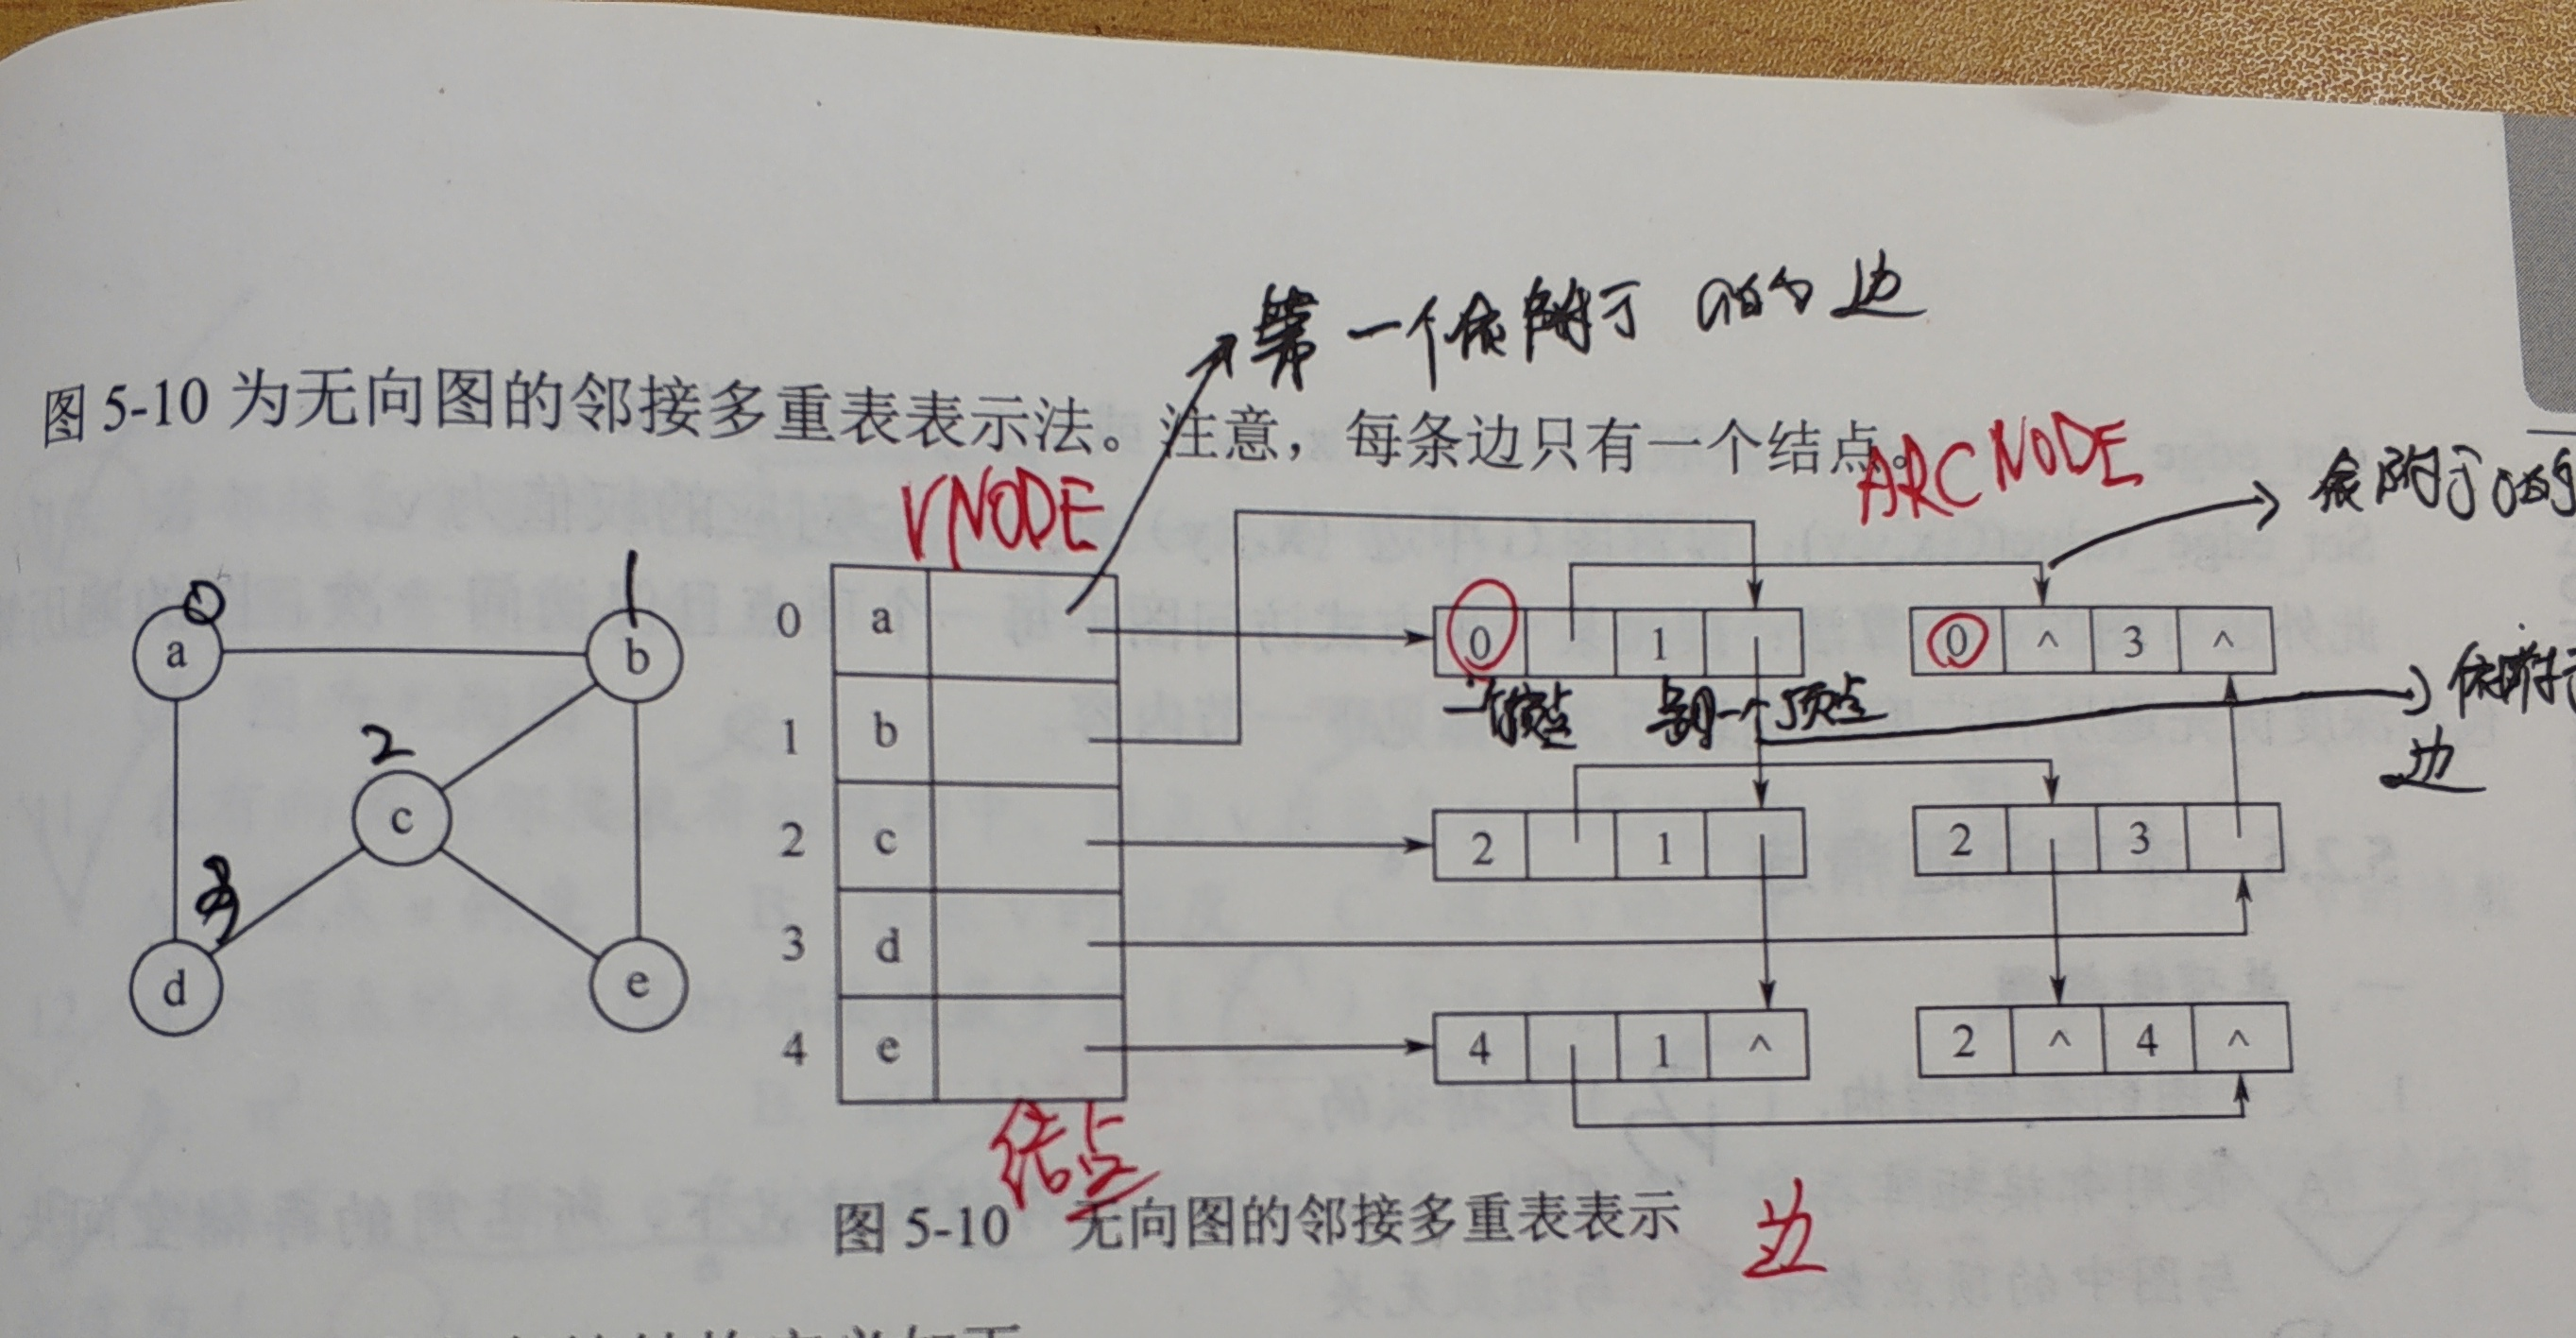
\includegraphics[scale=0.1]{example/chapter5/IMG_20181128_103024.png}
	\end{figure}
	\item 总共的空节点数量和顶点数量相同
\end{itemize}


\section{真题实战}


\subsection{2017年第3题}

\begin{figure}[H]
\centering  % 环境中的内容居中排版
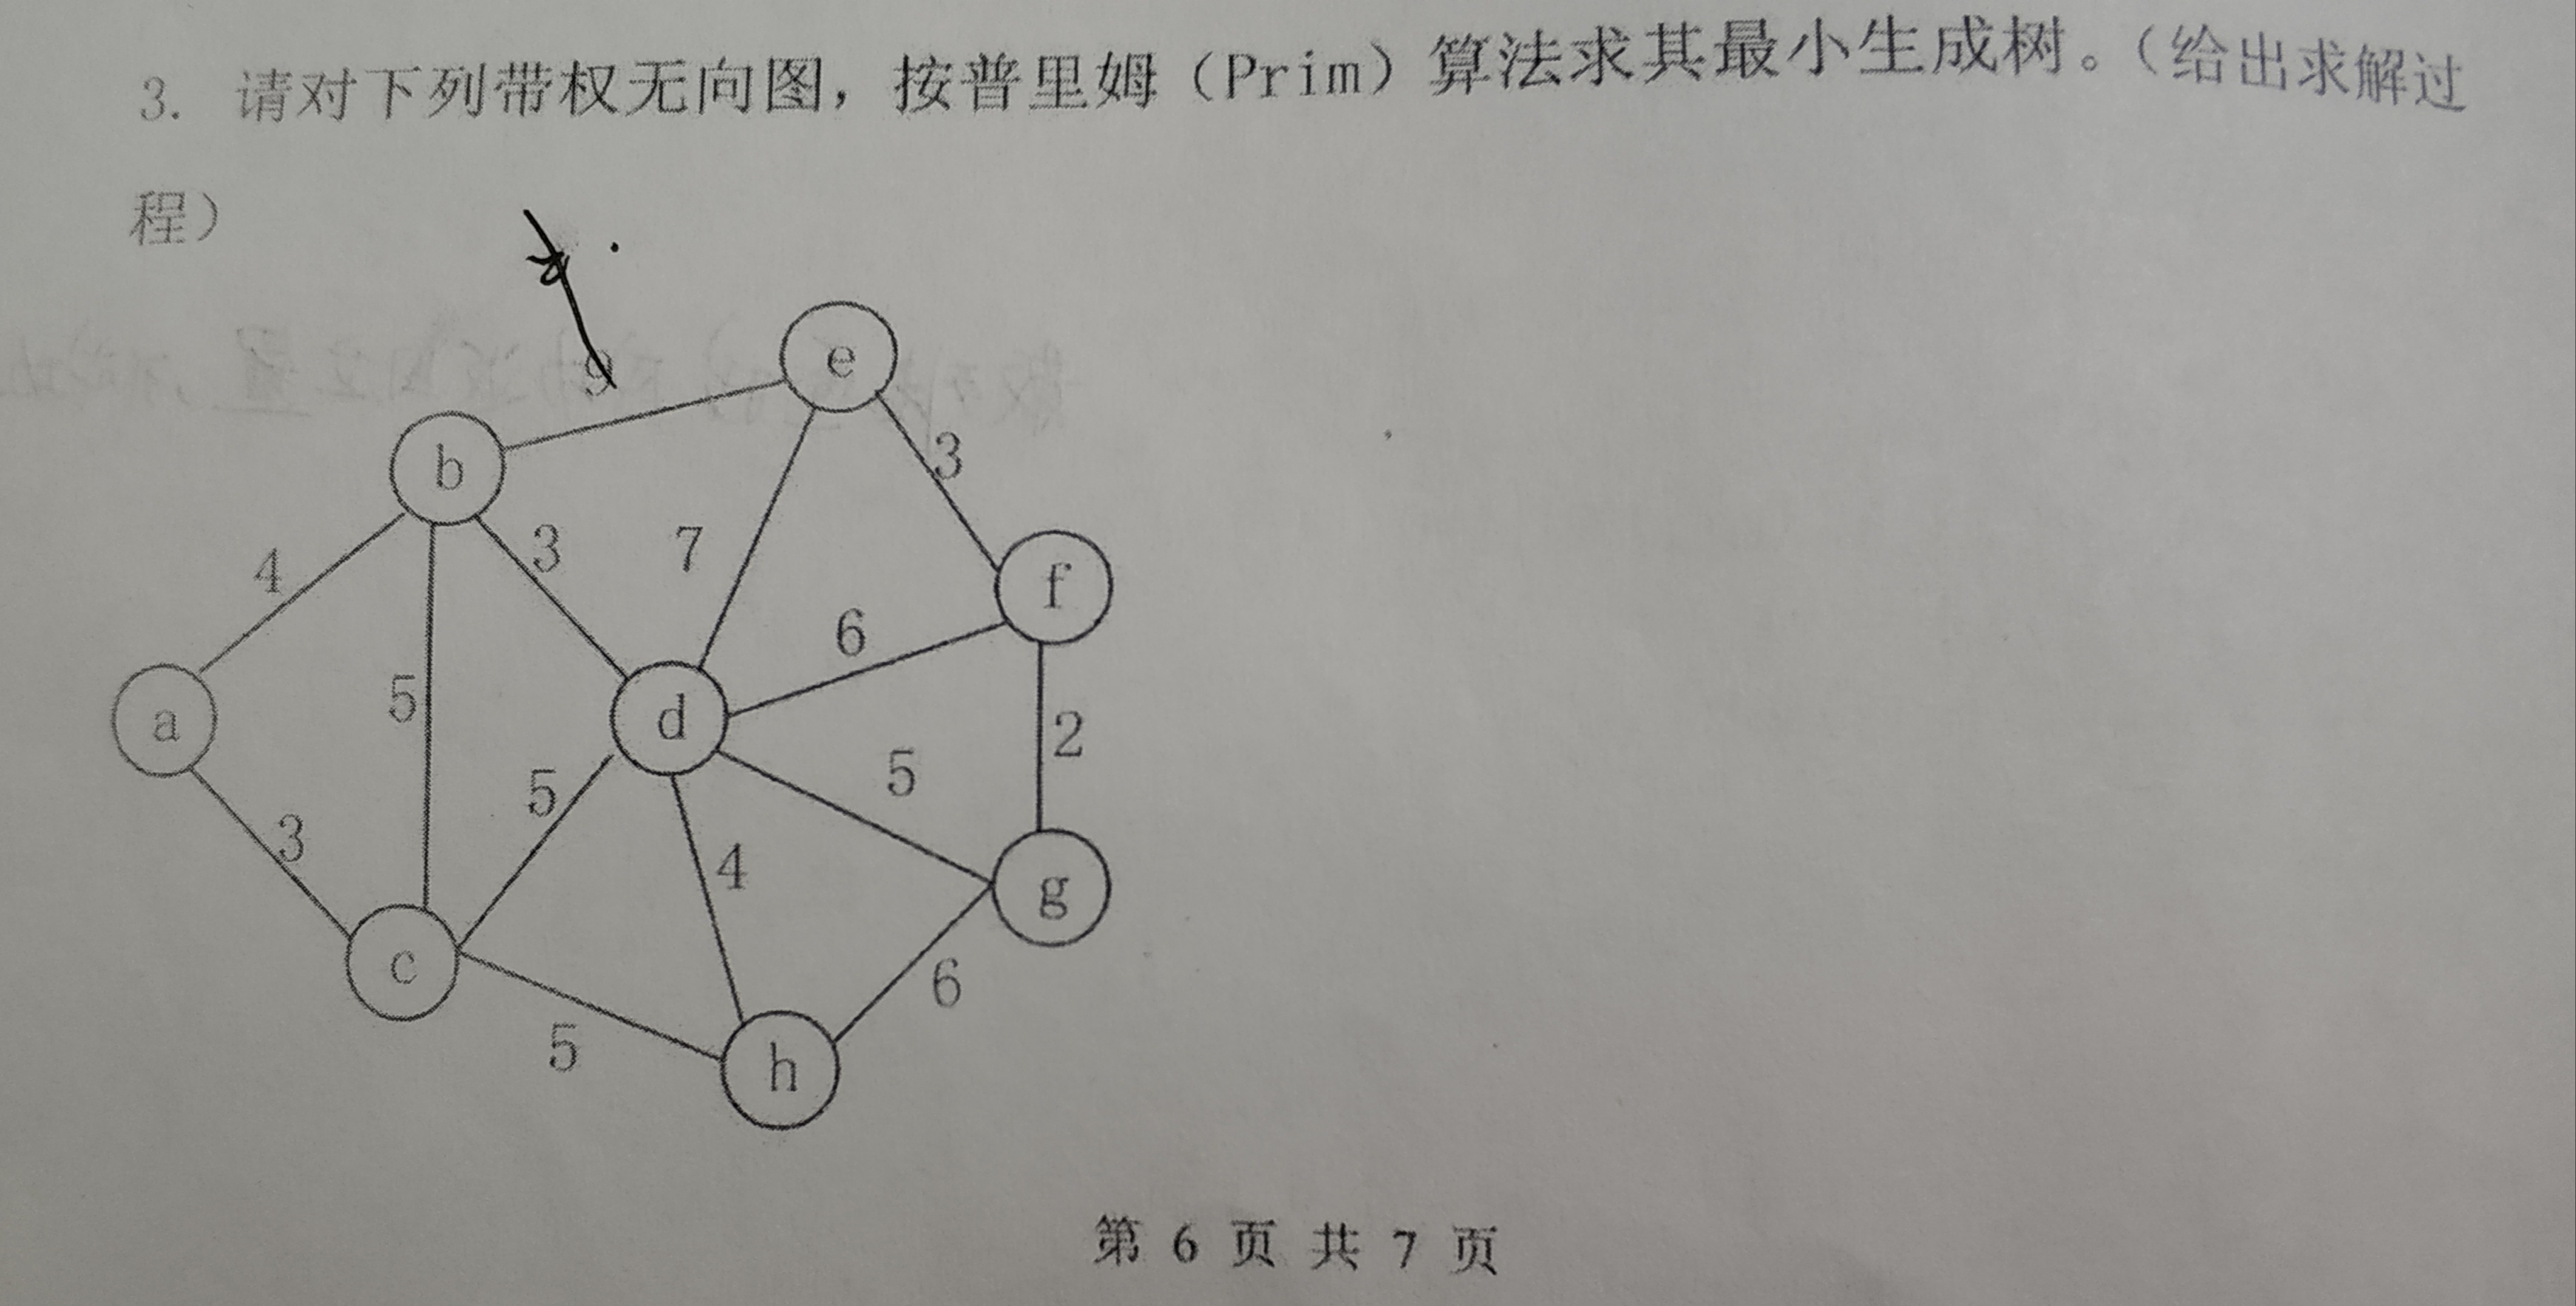
\includegraphics[scale=0.1]{example/chapter5/IMG_20181127_210442.png}
\end{figure}

解:\newline
严格按照严蔚敏的方式计算的话\newline
\begin{figure}[H]
\centering  % 环境中的内容居中排版
\includegraphics[scale=0.1]{example/chapter5/IMG_20181127_222510.png}
\end{figure}
注解  \newline
adjvex 那一行就是已经在生成树上的点到剩下的点最近的点\newline
下面紧挨着的就是距离,然后从中选出最短的距离,就是K值就是选中的点加入U集合\newline
一旦加入U集合下面就全部写0,U-K就是暂时不在生成树上的集合;\newline

\subsection{2016年(3)}
\begin{figure}[H]
\centering  % 环境中的内容居中排版
\includegraphics[scale=0.1]{example/chapter5/IMG_20181128_092826.png}
\end{figure}
解:\newline
~\\
1)\newline
\begin{lstlisting}[basicstyle=\small\ttfamily, caption={}, numbers=none]
Typedef struct ArcNode{
	Bool mark;
	Int ivex, jvex;
	Struct ArcNode *ilink,*jlink;
}ArcNode;
Typedef struct VNode{
	string data;                //顶点信息
	ArcNode *firstedge;
}VNode;
\end{lstlisting}
\begin{figure}[H]
\centering  % 环境中的内容居中排版
\includegraphics[scale=0.1]{example/chapter5/IMG_20181128_103404.png}
\end{figure}
2)\newline
\begin{figure}[H]
\centering  % 环境中的内容居中排版
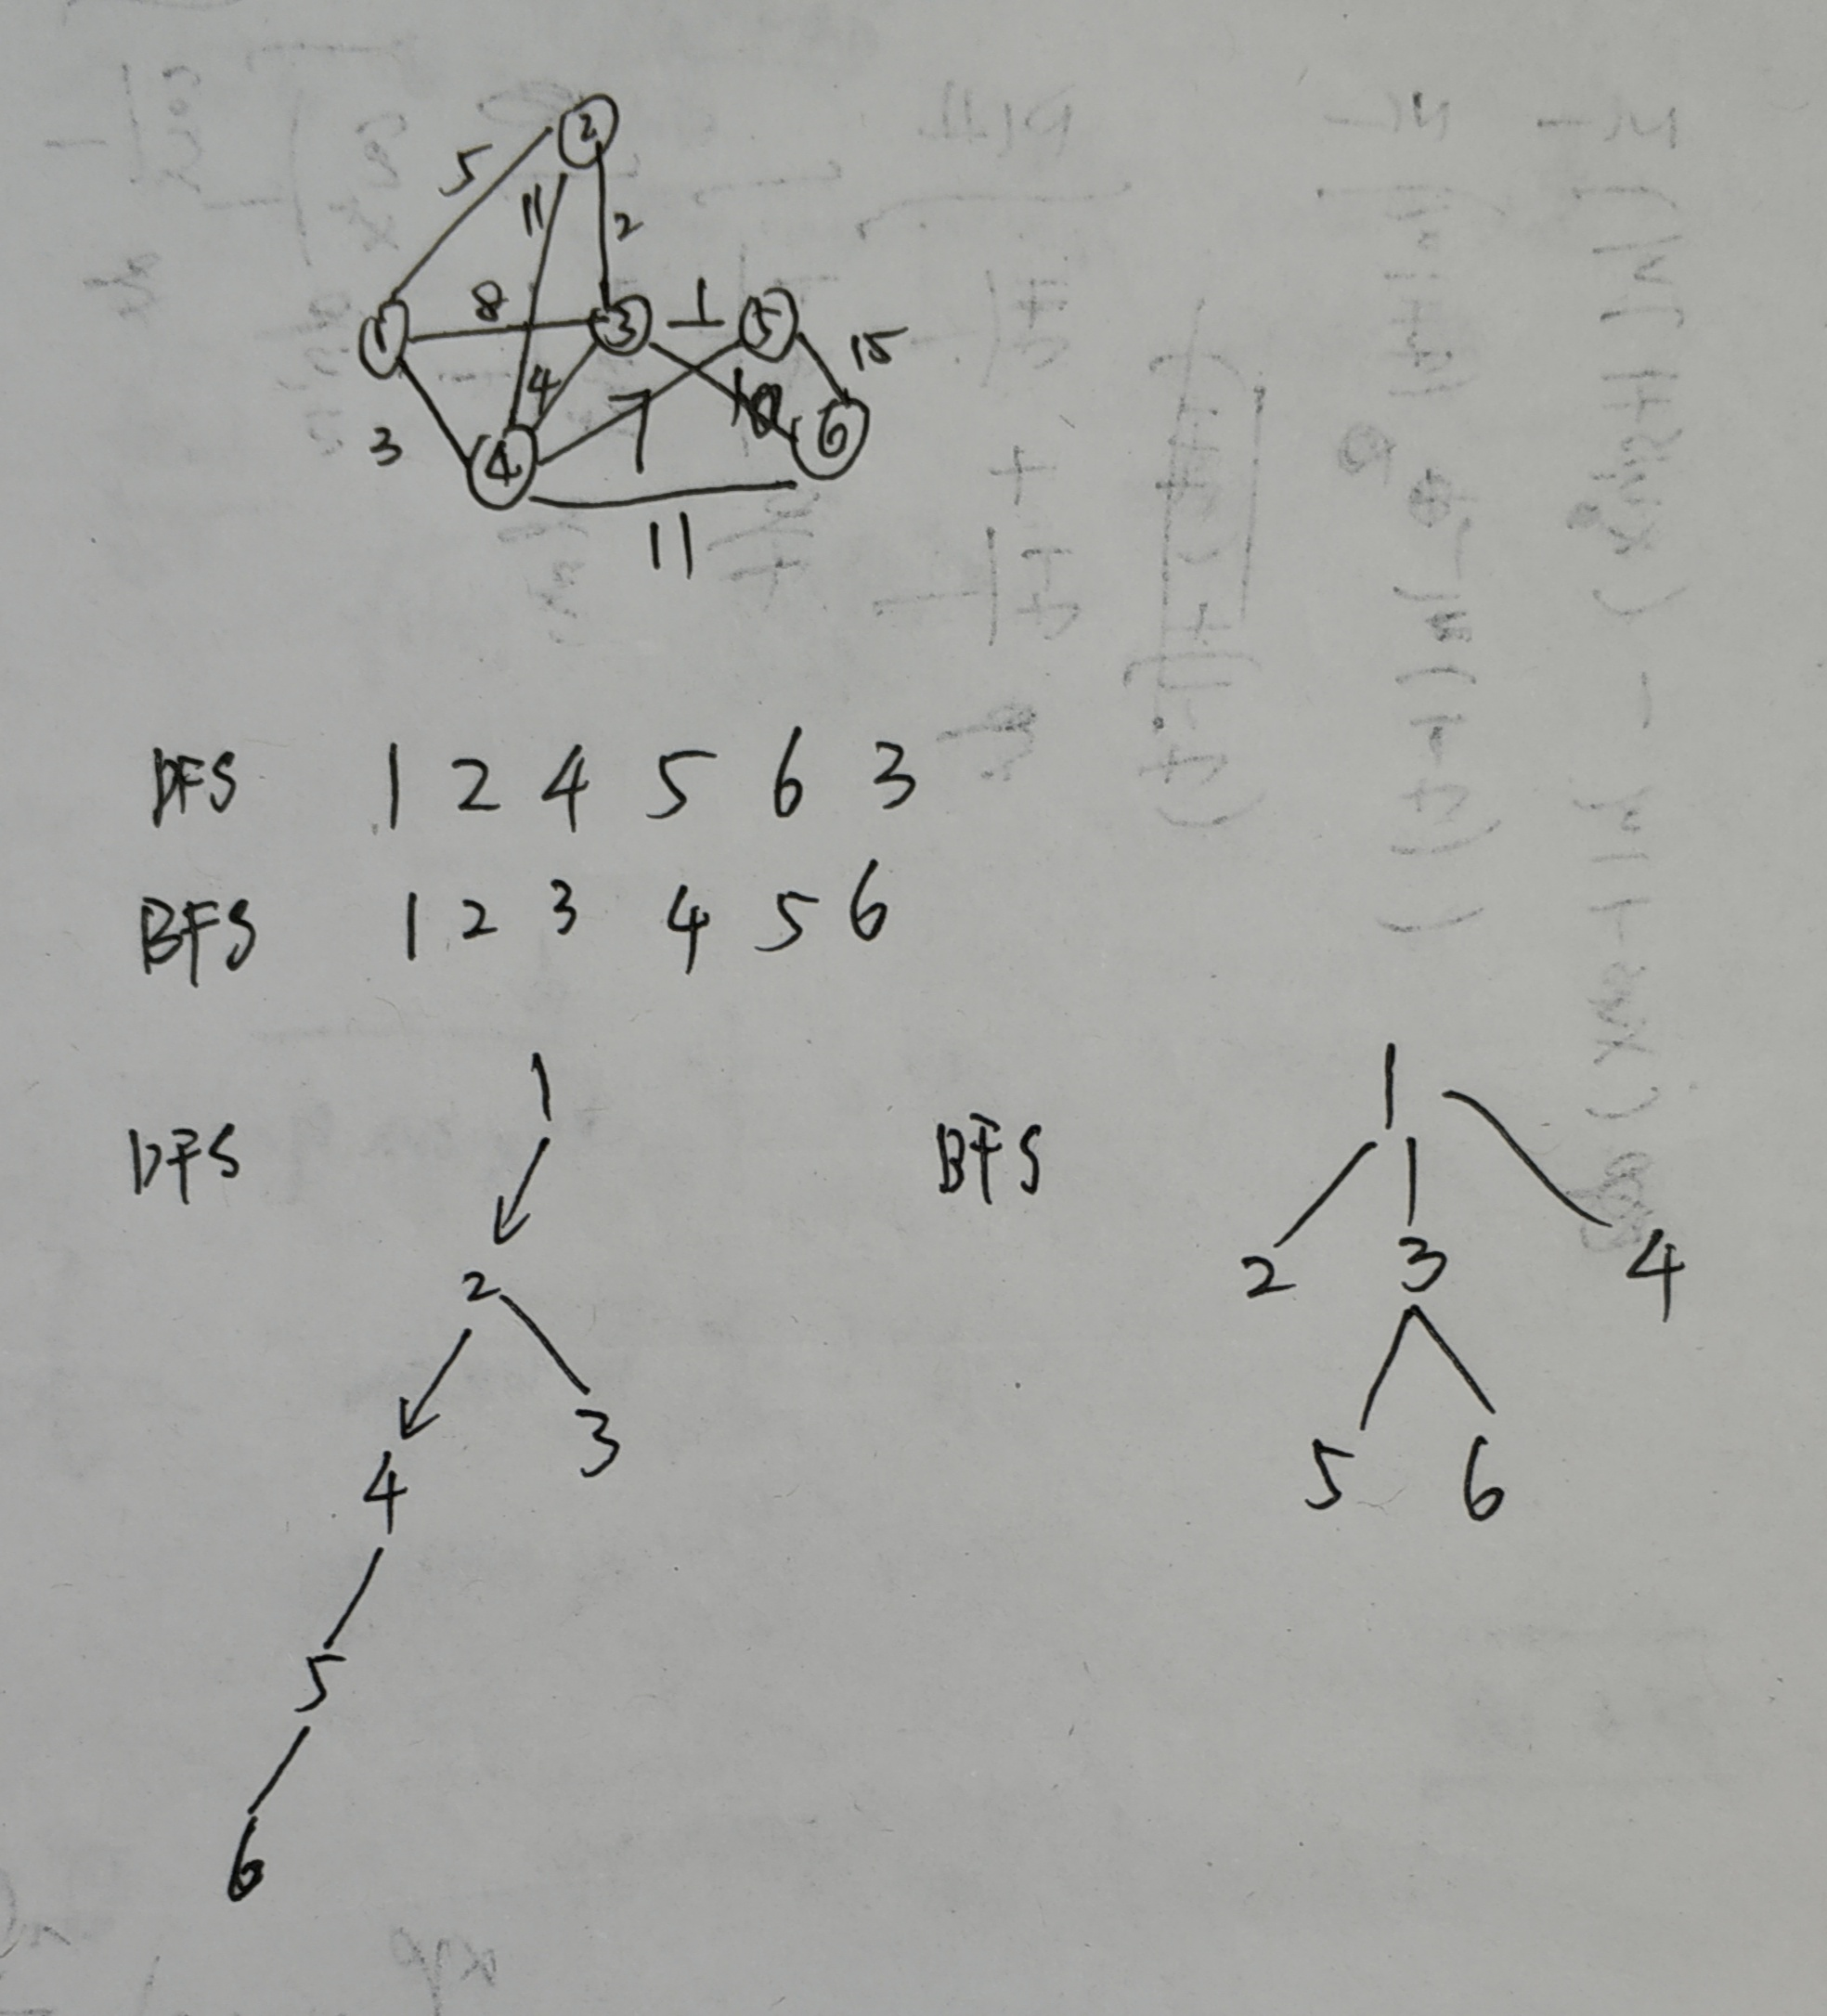
\includegraphics[scale=0.1]{example/chapter5/IMG_20181128_110619.png}
\end{figure}
3)\newline
最小生成树的边集{1,4},{1,2},{2,3},{3,5},{3,6} \newline
\begin{figure}[H]
\centering  % 环境中的内容居中排版
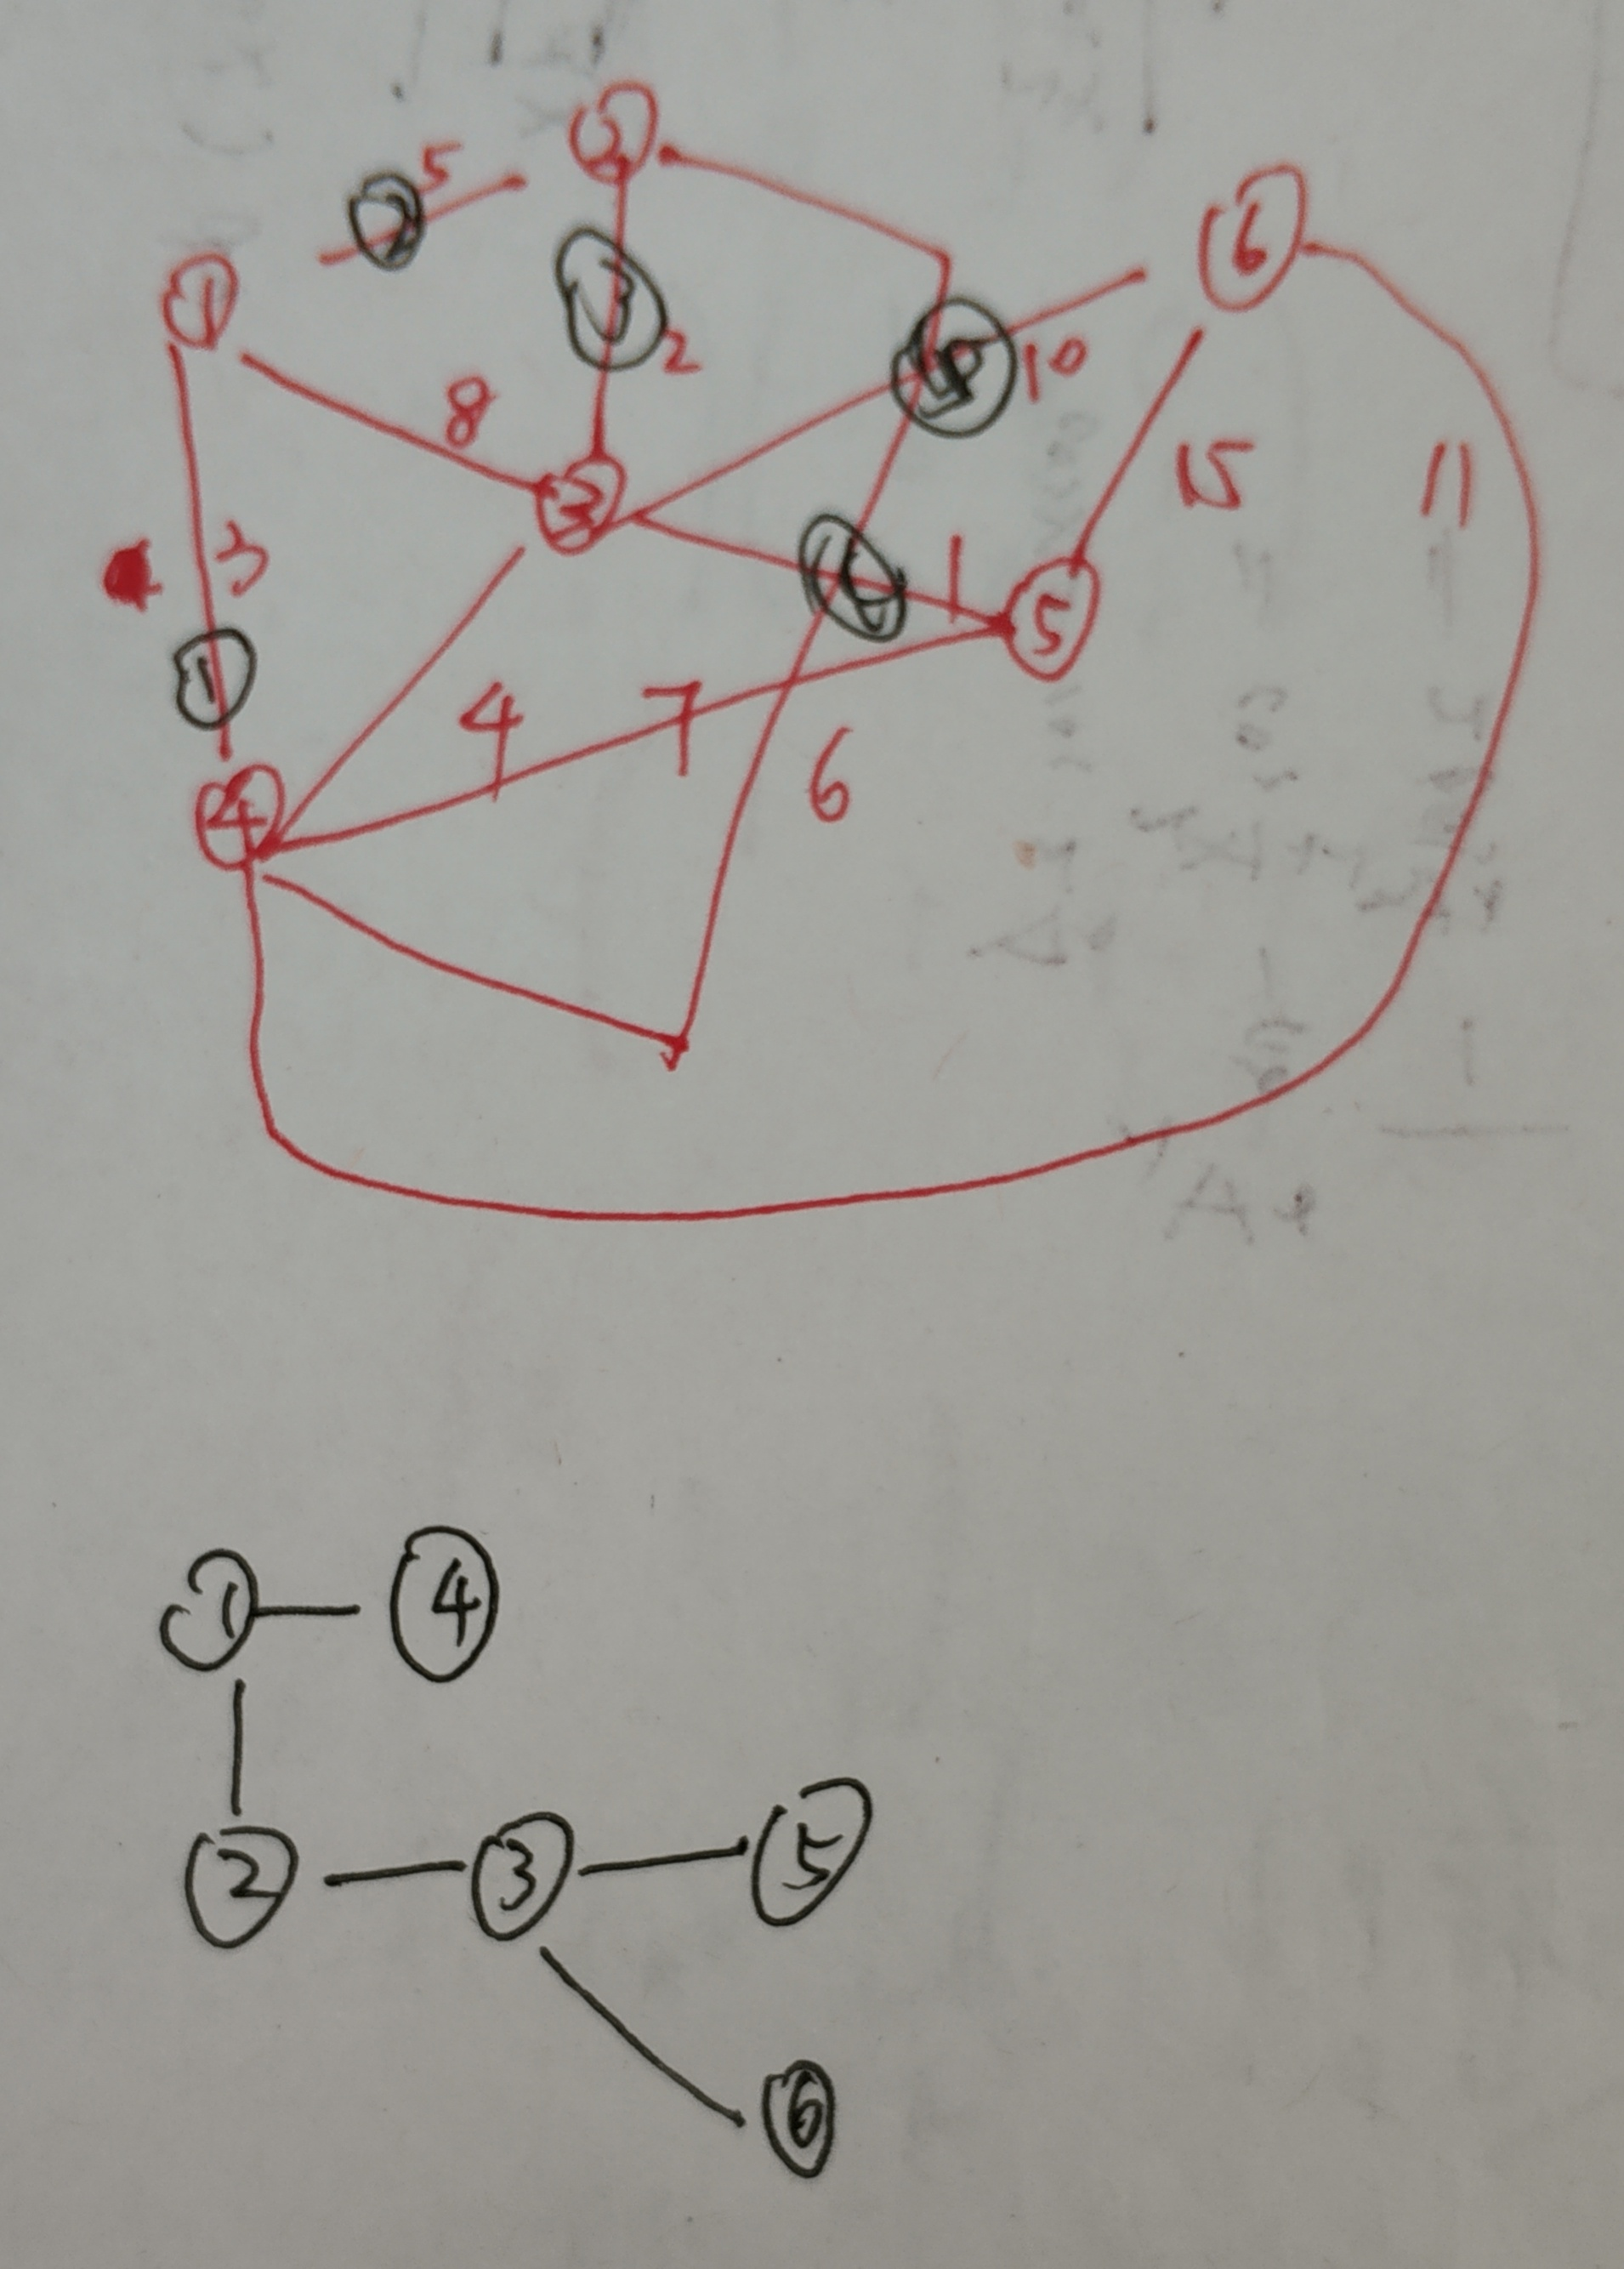
\includegraphics[scale=0.1]{example/chapter5/IMG_20181128_111203.png}
\end{figure}

\subsection{2014年第5题}


\begin{figure}[H]
\centering  % 环境中的内容居中排版
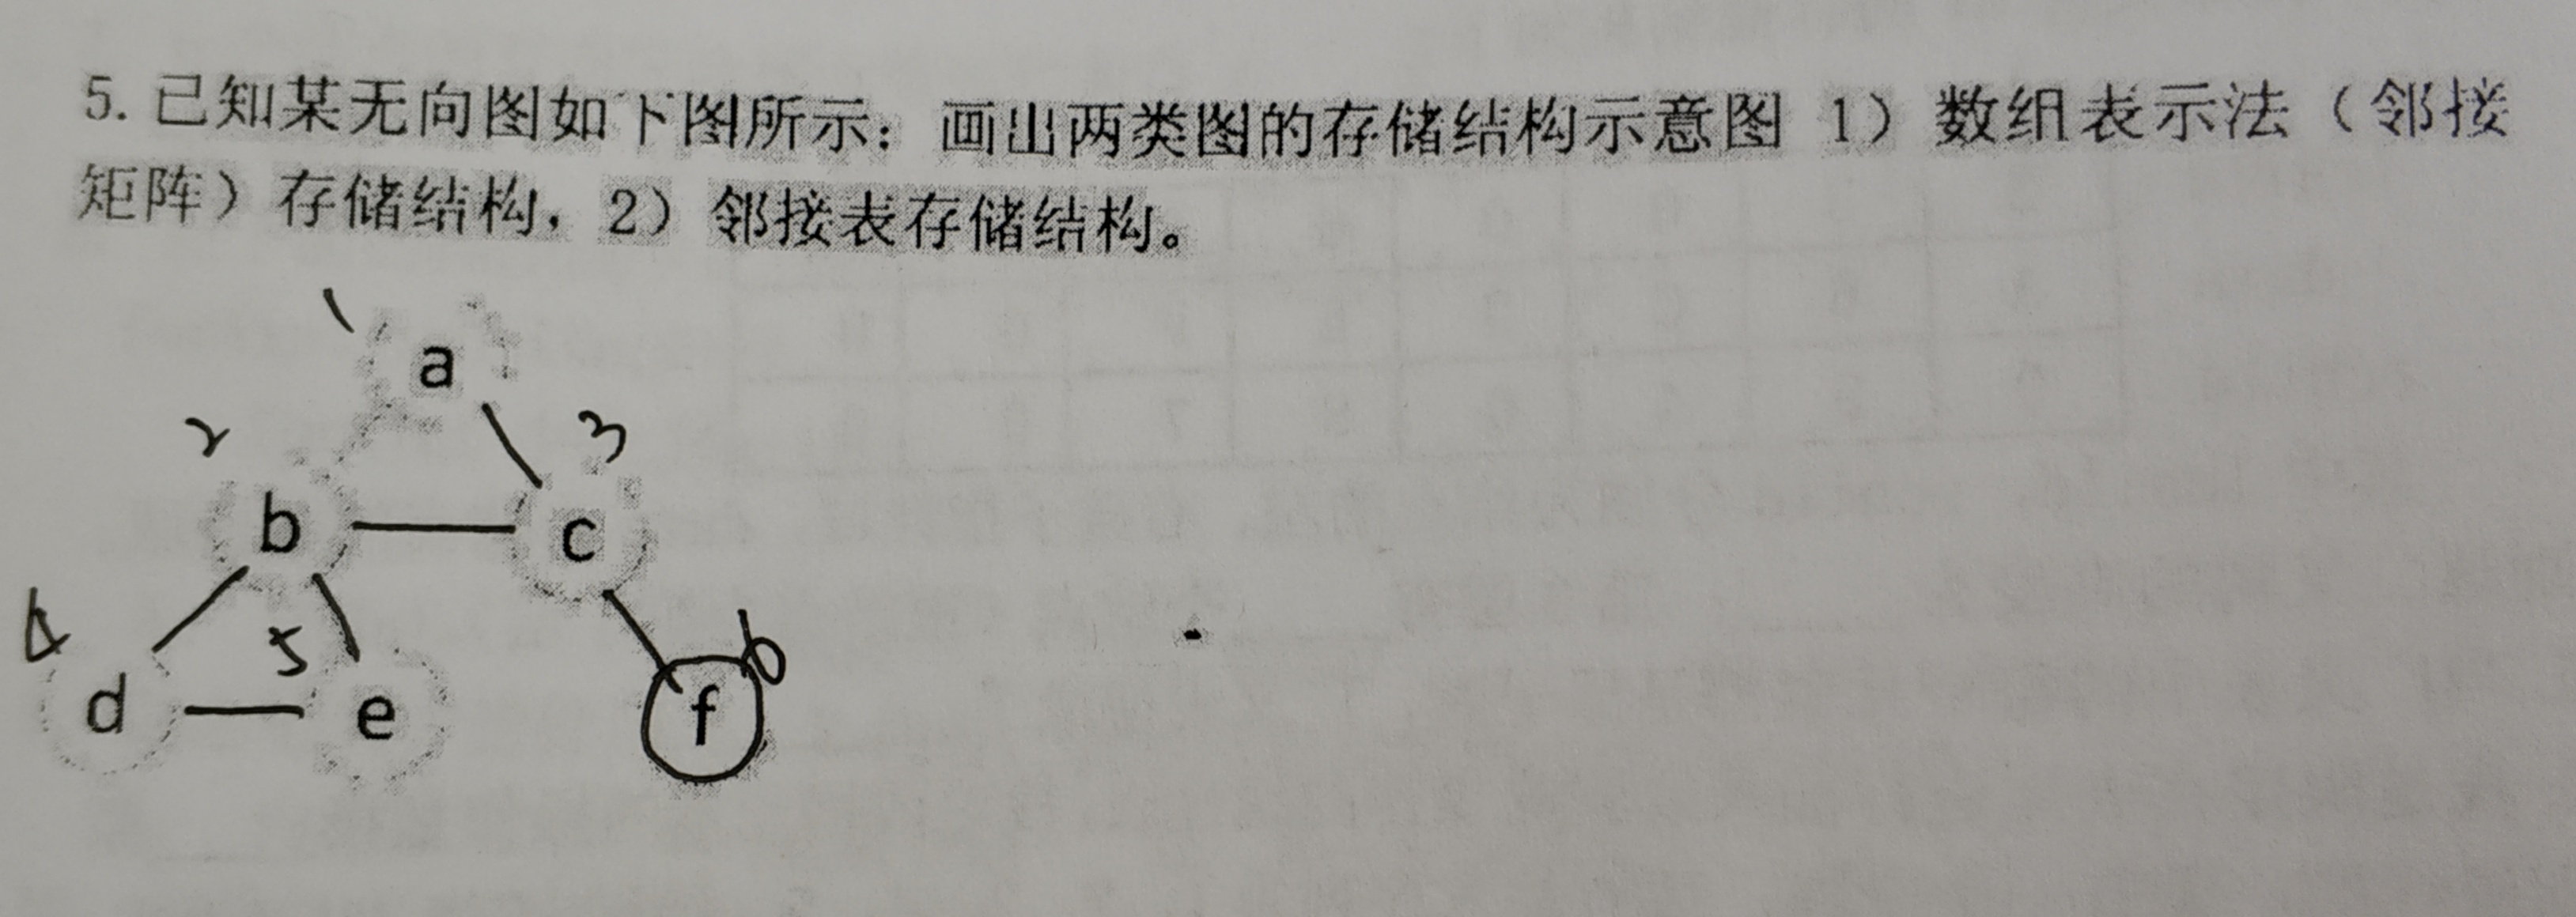
\includegraphics[scale=0.1]{example/chapter5/IMG_20181128_134713.png}
\end{figure}

解:\newline

\begin{figure}[H]
\centering  % 环境中的内容居中排版
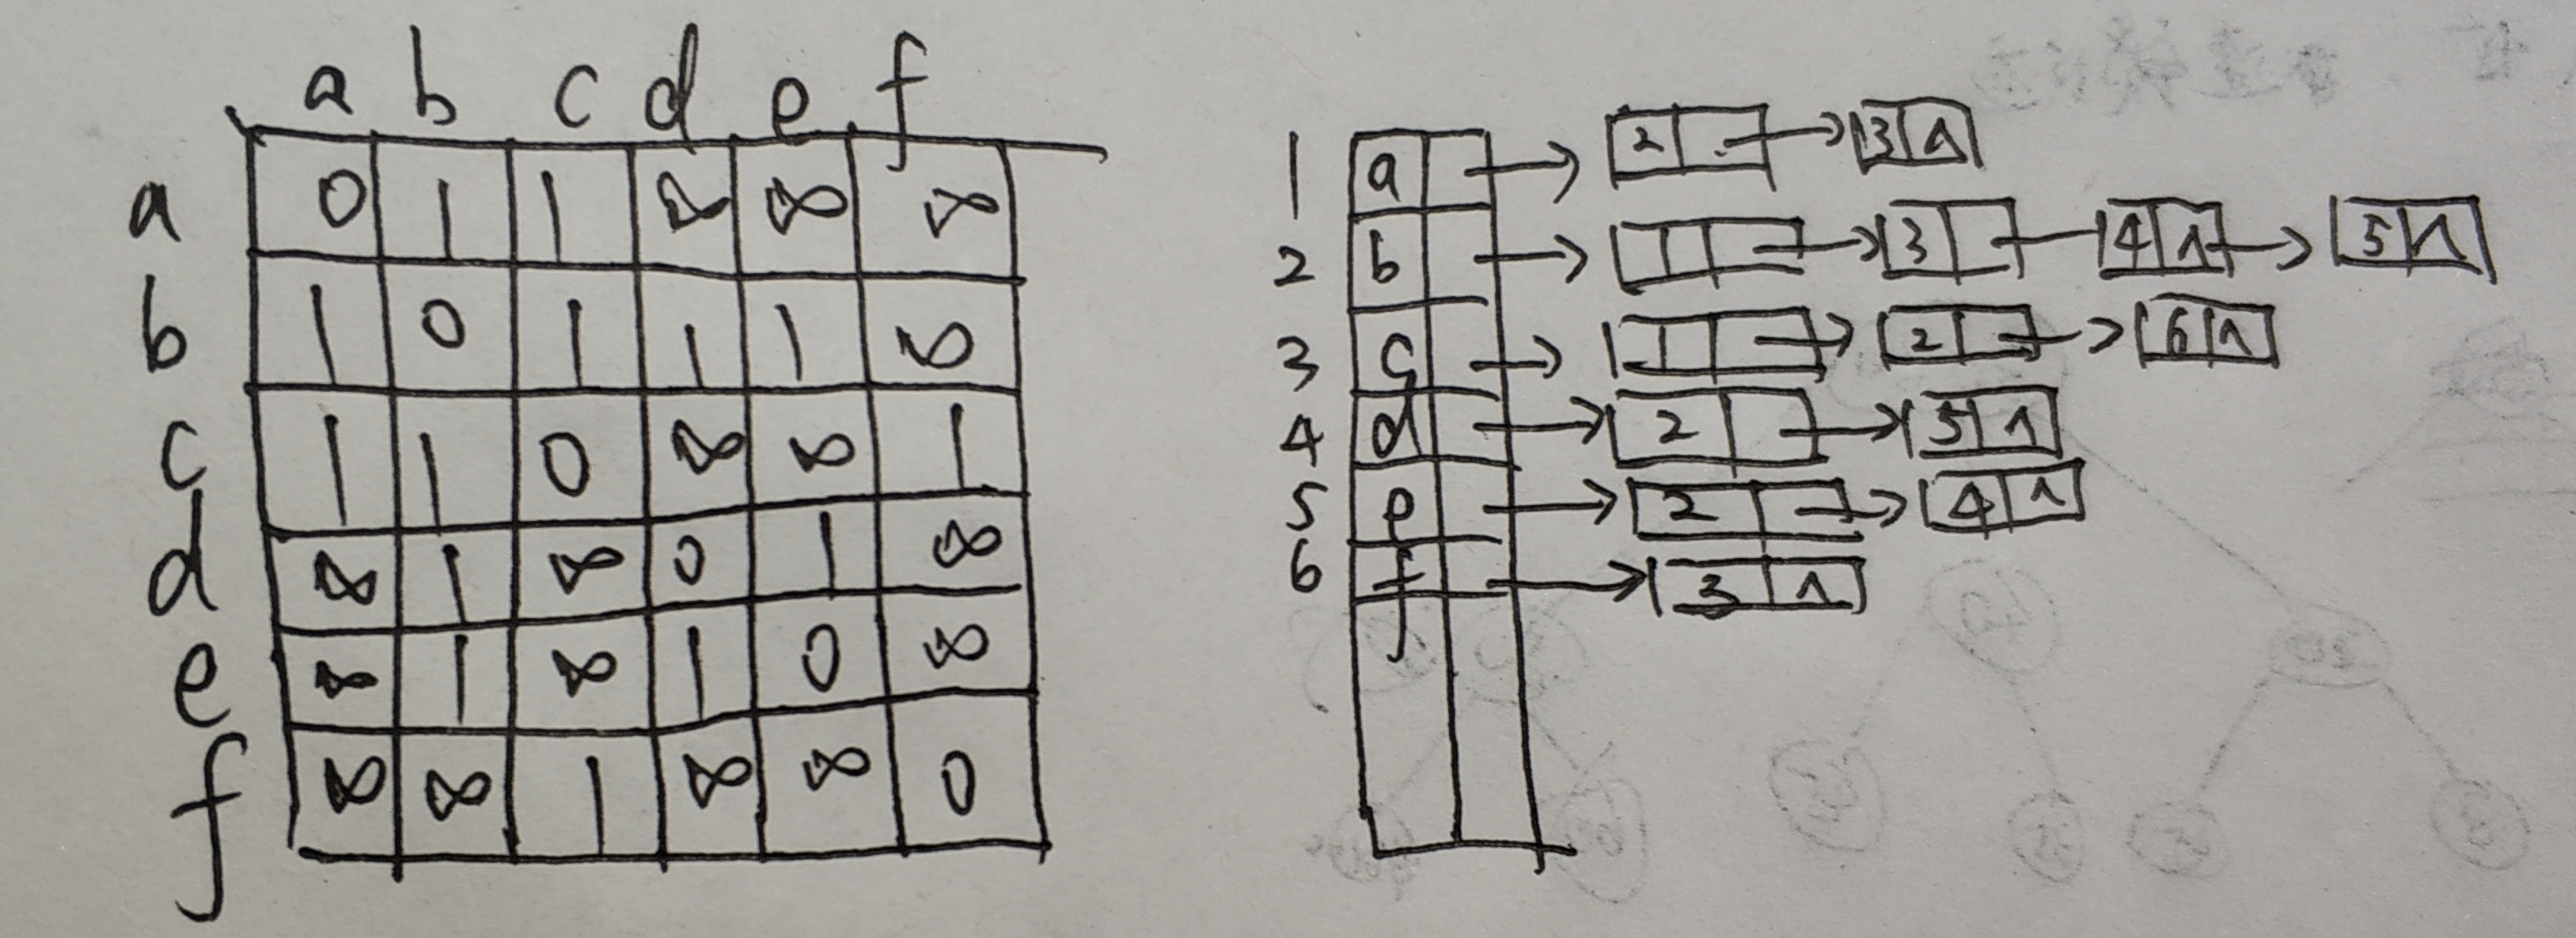
\includegraphics[scale=0.1]{example/chapter5/IMG_20181128_134745.png}
\end{figure}